\documentclass[11pt,a4paper,oneside, reqno]{amsproc}
\usepackage{changepage}
\usepackage{mathtext} % русские буквы в формулах
\usepackage[T2A]{fontenc}
\usepackage[utf8x]{inputenc}
\usepackage{ucs}
\usepackage{cmap}
\usepackage[english,russian]{babel}
\usepackage{graphicx}
%\usepackage{concrete}
%\usepackage{amsmath}
%\usepackage{amsfonts}
\usepackage{amssymb}
\usepackage{dcolumn}
\usepackage{booktabs}
\usepackage{ctable}
\usepackage{multirow}

\newcommand{\specialcell}[2][c]{%
  \begin{tabular}[#1]{@{}c@{}}#2\end{tabular}}
\oddsidemargin = 0pt
\textwidth = 14 cm
\topmargin = -2 cm
\textheight = 24 cm
\makeatletter
\renewcommand{\theequation}{\thesection.\arabic{equation}}
\@addtoreset{equation}{section}
\newcommand{\eq}{\begin{equation}}
\newcommand{\eeq}{\end{equation}}
\newcommand{\fr}{\frac}
\newcommand{\mf}{\mathfrak}
\newcommand{\sub}{\subsection}
\newcommand{\subsub}{\subsubsection}
\newcommand{\definition}{\theoremstyle{definition}}
\newcommand{\mult}[2]{\genfrac{\left[}{\right.}{0pt}{}{#1}{#2}}
\renewcommand{\qed}{\begin{center} $\mathsf{QED}$ \end{center}}
\newcommand{\al}{\alpha}
\newcommand{\comment}[1]{\marginpar{\Small{{\sl #1}}} }
\newcommand{\epigraph}[2]{\begin{flushright} {\em #1}\\#2\\[20 pt]
\end{flushright}}
\newcommand{\fx}[1]{\ensuremath{\mathit{f}_{#1}(x)}}
\newcommand{\re}[1]{(\ref{#1})}
\newcommand{\mh}{\mathit}
\newcommand{\itm}[1]{\begin{itemize}	\item #1 \end{itemize}}
\newcommand{\note}[1]{\begin{flushleft}\hbox{%
\vrule\hspace{.5em}\parbox{ .9\textwidth}%
{ #1}} \end{flushleft}}
\newcommand{\Al}{\ensuremath{\mathcal{A}}}
\newcommand{\@dotsep}{3.9}
\newcommand{\system}[1]{\eq\left\{ \begin{aligned} #1
\end{aligned}\right.\\[5 pt]\eeq}
\renewcommand{\phi}{\varphi}

% http://www.texnik.de/floats/caption.phtml
% This does spacing around caption.
%\setlength{\abovecaptionskip}{6pt}   % 0.5cm as an example
%\setlength{\belowcaptionskip}{9pt}   % 0.5cm as an example

%%%%%%%%%%%%%%%%%%%%%%%%%%%%%%%%%%%%%%%%%%%%%%%%%%%%%%%%%%%%%%%%%%%%%%%

\author{Соколовский Роман}
\begin{document}

\begin{titlepage}
    \begin{center}
        \textsc{\large Санкт-Петербургский Государственный Университет Аэрокосмического Приборостроения}\\[5cm]
        \rule{\textwidth}{1pt}\\
        \vspace{10pt}
        { \huge \bfseries Исследование Дисперсии и Затухания
        Волн в Волноводе Прямоугольного Печения с $H_{10}$.}\\[0.4cm]
        \hrule
        \vspace{0.4cm}
        \textsc{ {\large Отчет по Лабораторной работе №7}}
        
        \vspace{2.5cm}
        \begin{flushright}
        \begin{minipage}{0.5\textwidth}
            \begin{flushright} 
                \textsc{\small Выполнил}:\\
                \large
                Студент факультета №\textbf{5}\\
                Группы \textbf{5025} кафедры \textbf{52}\\[2pt]
                \textsc{Соколовский} \textsc{Р}оман \textsc{А}лександрович
            \end{flushright}
        \end{minipage}
        \end{flushright}
        \vfill
        {\large Санкт-Петербург\\2012}
    \end{center}
\end{titlepage}

\section{Цель Работы}
\begin{itemize}
    \item Изучение явления дисперсии и затухания волн в волноводе.
    \item Изучение методов измерения параметров, характеризующих 
        дисперсию и затухание.
    \item Экспериментальное исследование изменения фазовой и групповой
        скоростей, а также затухания в зависимости от частоты
        генерируемых колебаний.
    \item Исследование математической зависимости затухания, фазовой и
        групповой скоростей от поперечных размеров волновода, 
        диэлектрической проницаемости заполнения и удельной проводимости
        стенок в заданном частотном диапазоне.\\
\end{itemize}

\section{Схема Лабораторной Установки}
Схема лабораторной установки представлена на Рис. \ref{fig:scheme}.
\begin{figure}[h!]
    \begin{center}
        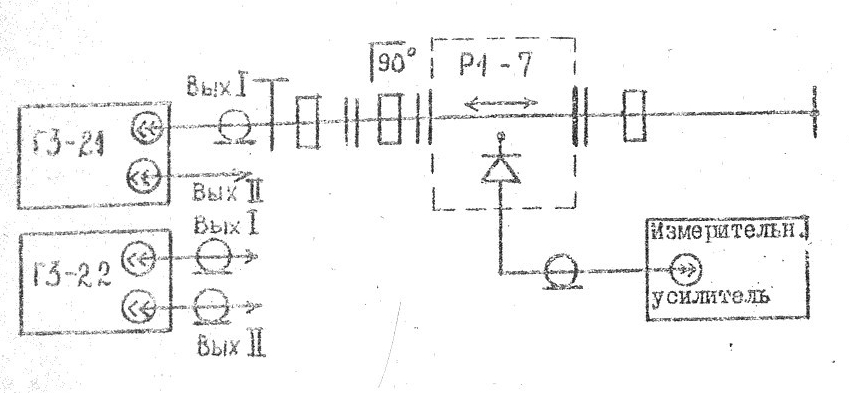
\includegraphics[width=\textwidth]{scheme.jpg}
    \end{center}
    \vspace{-20pt}
    \caption{Принципиальная схема лабораторной установки}
    \label{fig:scheme}
\end{figure}

\newpage
\section{Результаты измерений и вычислений}
\subsection{Измерения и вычисления}
\subsubsection{Теоретический коэффициент затухания $\alpha_{H_{10}}$.}
\begin{equation}
    \alpha_{H_{10}} = \frac{0.793\left[ 1 + 2\frac{b}{a}\left( \frac{\lambda}{2a} \right)^2\right]}
                            {b\sqrt{\sigma\lambda \left[ 1 - \left( \frac{\lambda}{2a} \right)^2\right]}}
    \label{eq:alpha_teor}
\end{equation}
\vspace{10 pt}

\subsubsection{Экспериментальный коэффициент затухания $\alpha_{H_{10}}$.}
\begin{equation}
    \alpha_{H_{10}} = 8.686 \frac{КБ_v}{l}
    \label{eq:alpha_pract}
\end{equation}

\begin{equation}
    КБ_v = \frac{\pi\cdot \Delta z}{\Lambda}
    \label{eq:kbv}
\end{equation}

\begin{equation}
    \Lambda = 2 (l_{2\min} - l_{1\min} ) 
    \label{eq:Lambda}
\end{equation}

\begin{equation}
\lambda = \frac{\Lambda}{\sqrt{1 +
            \left( \frac{\Lambda}{2a} \right)^2}}
\end{equation}

\subsection{Таблицы результатов измерений и вычислений}
Экспериментальные характеристики электромагнитной волны в волноводе
сведены в Таблицу~\ref{tab:tab1}. Теоретические величины 
представлены в Таблице~\ref{tab:tab2}.\\

\begin{centering}
\begin{table}[h!]
\newcolumntype{W}{D{.}{.}{2.3}}
%\begin{adjustwidth}{-1.5cm}{}
\vspace{10pt}
\begin{tabular}{ccccccccccccc} \toprule %[-2.08em]
\newcolumntype{W}{D{.}{.}{2.3}}
$f$, MHz  &  $z_1$   &  $z_2$   &  $z_1'$  &  $z_2'$  &  $l_1$    &  $l_2$    &  $L$     &  $\lambda$   &  $KB_v$     &  $\alpha$    &  $V_{gr}/c$    &  $V_{ph}/c$    \\
 \midrule
3000  &  1.4  &  1.7  &  8.6  &  8.3  &  1.55  &  8.45  &  13.8  &  9.92  &  20.4  &  59.20  &  0.72  &  1.38  \\
3200  &  0.5  &  2.3  &  6.6  &  8.4  &  1.4   &  7.5   &  12.2  &  9.27  &  4.29  &  12.44  &  0.75  &  1.32  \\
3600  &  2.3  &  3.3  &  7.3  &  8.4  &  2.8   &  7.85  &  10.1  &  8.24  &  8.38  &  24.26  &  0.81  &  1.22  \\
4000  &  1.5  &  1.6  &  5.8  &  5.9  &  1.55  &  5.85  &  8.6   &  7.36  &  27.4  &  79.34  &  0.85  &  1.16  \\
4200  &  1.9  &  2.0  &  6.1  &  6.2  &  1.95  &  6.15  &  8.4   &  7.24  &  27.2  &  78.90  &  0.86  &  1.16  \\
\bottomrule
\end{tabular}
\vspace{5 pt}
\caption{Экспериментальные характеристики.} 
%\end{adjustwidth}
\label{tab:tab1}
\end{table}
\end{centering}

\begin{centering}
\begin{table}[h!]
\newcolumntype{W}{D{.}{.}{2.3}}
%\begin{adjustwidth}{-1.5cm}{}
\vspace{10pt}
\begin{tabular}{ccccccccccccc} \toprule %[-2.08em]
\newcolumntype{W}{D{.}{.}{2.3}}
$f$, MHz  &  $\lambda$  &  $\Lambda$  &  $V_{gr}/c$  &  $V_{ph}/c$  &  $\alpha$  &  $\alpha$, dB/m  \\
 \midrule
3000  &  0.1    &  0.138  &  0.71  &  1.39  &  0.0197  &  34.11  \\
3200  &  0.093  &  0.124  &  0.75  &  1.32  &  0.0186  &  34.61  \\
3600  &  0.083  &  0.102  &  0.81  &  1.23  &  0.0172  &  35.29  \\
4000  &  0.075  &  0.087  &  0.85  &  1.17  &  0.0165  &  35.65  \\
4200  &  0.071  &  0.082  &  0.86  &  1.15  &  0.0164  &  35.70  \\
\bottomrule
\end{tabular}
\vspace{5 pt}
\caption{Теоретические характеристики.} 
%\end{adjustwidth}
\label{tab:tab2}
\end{table}
\end{centering}

\subsection{Графики и рисунки}
На основе данных таблиц~\ref{tab:tab1},~\ref{tab:tab2} были построены сравнительные характеристики
теоретических и практических зависимостей фазовой и групповой скоростей (Рис.~\ref{fig:plot1}), а также коэффициента
затухания электромагнитной волны (Рис.~\ref{fig:plot2}).

\begin{figure}[hb!]
    \begin{center}
        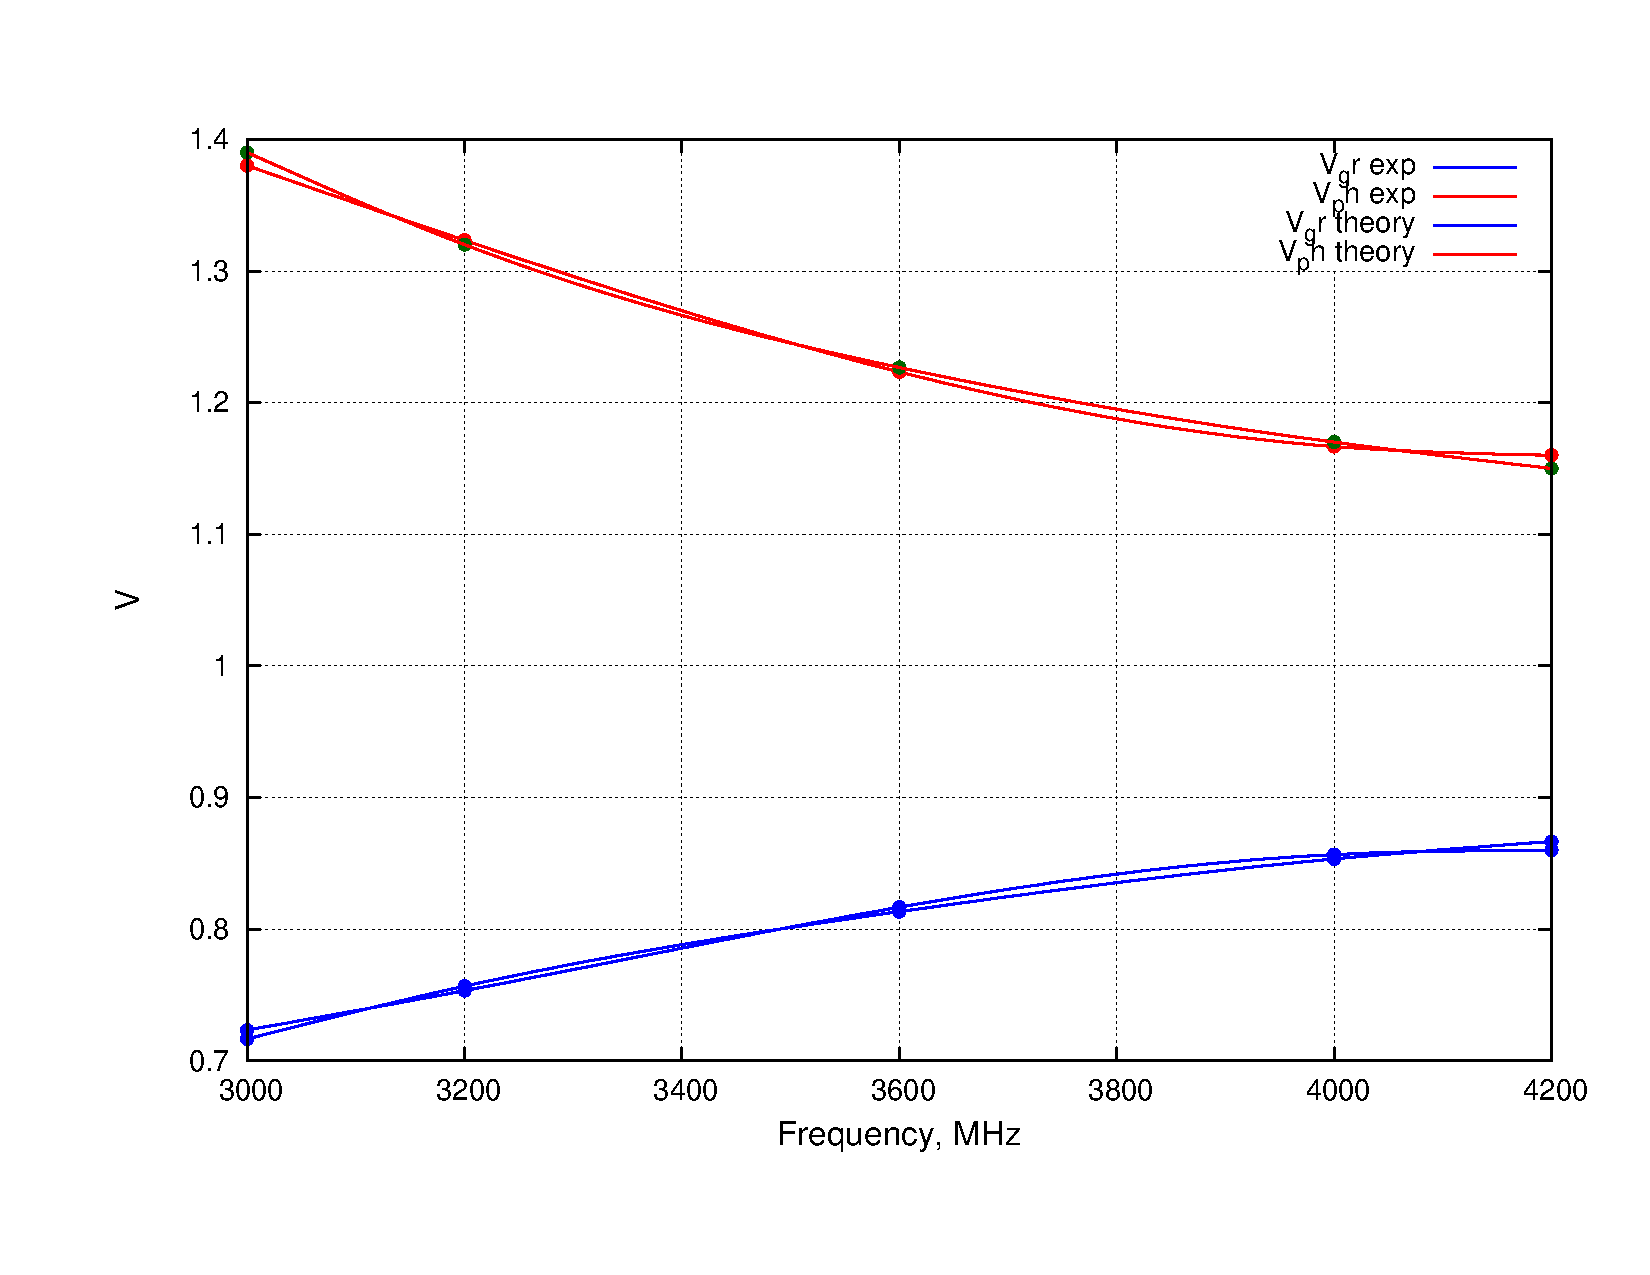
\includegraphics[width=\textwidth]{plot1.pdf}
    \end{center}
    \caption{График зависимости фазовой и групповой скоростей от частоты.}
    \label{fig:plot1}
\end{figure}

\begin{figure}[h!]
    \begin{center}
        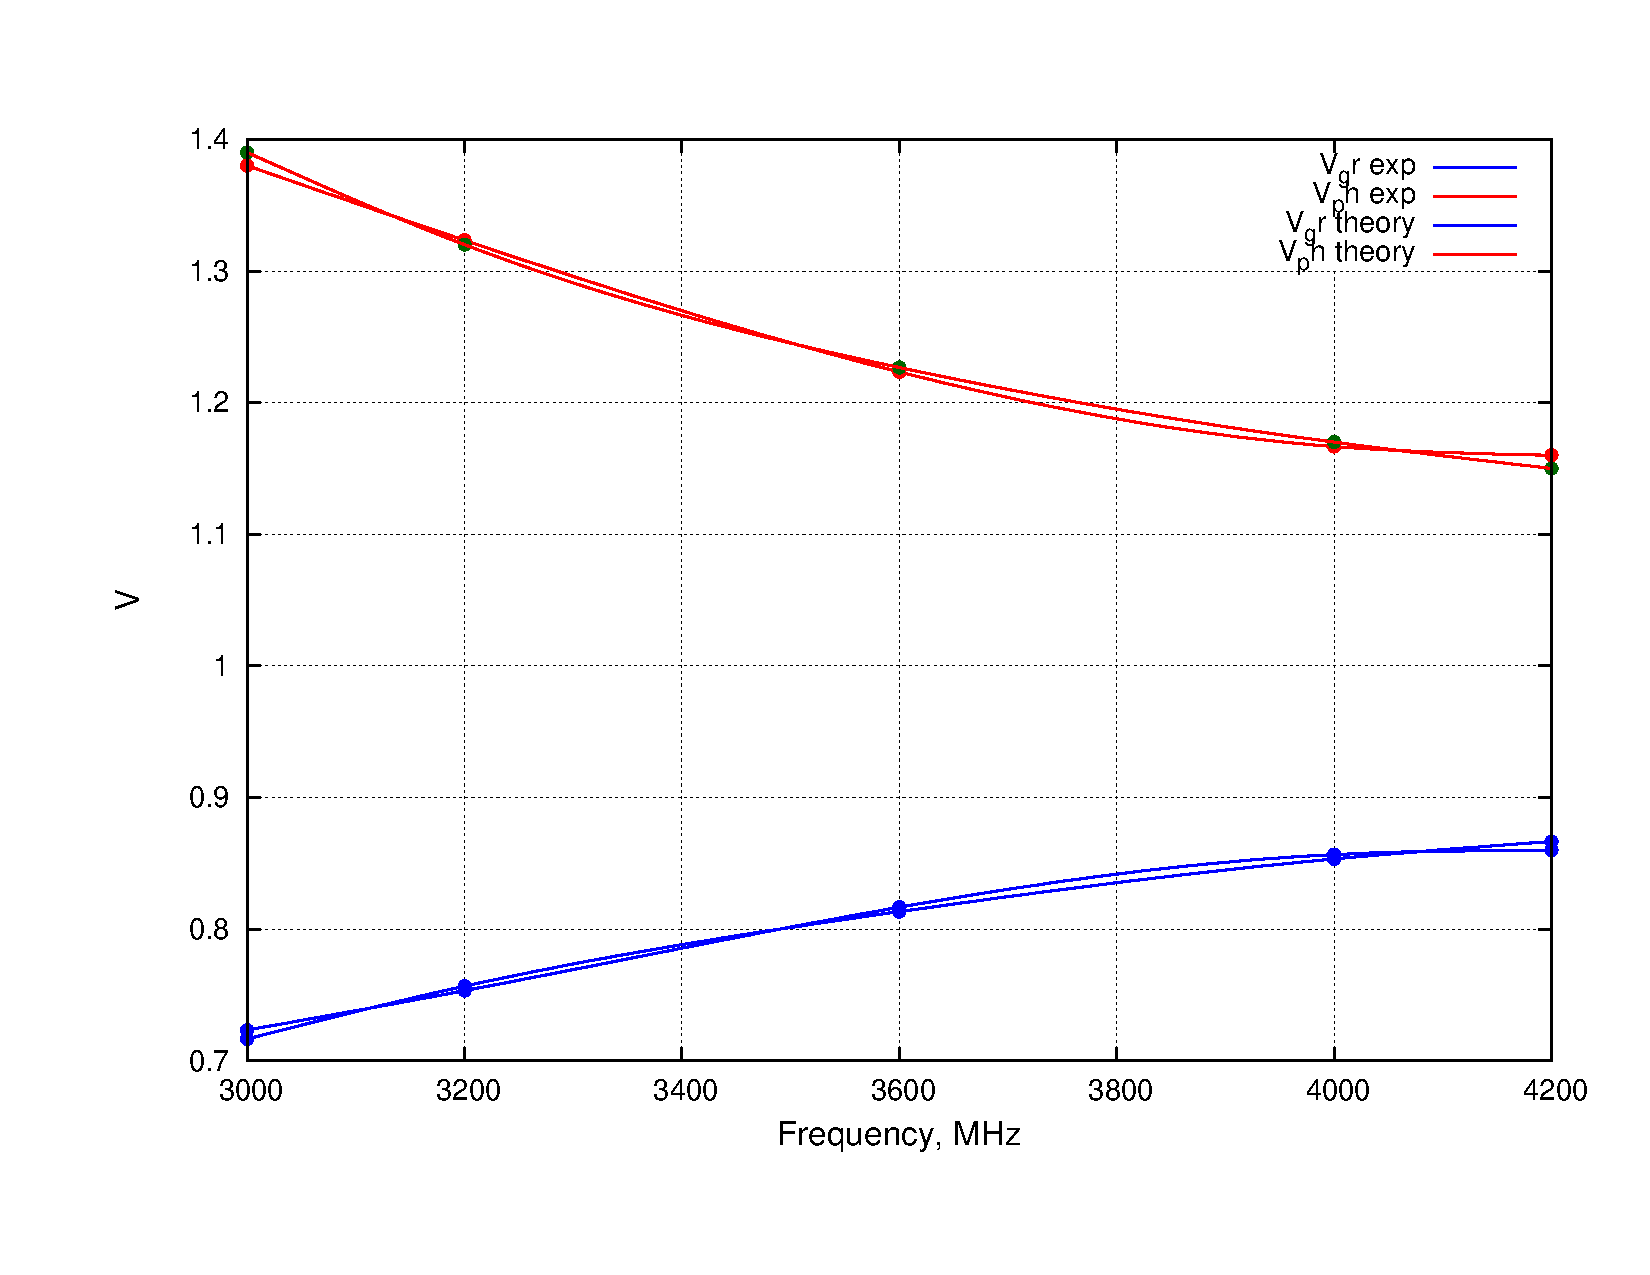
\includegraphics[width=0.7\textwidth]{plot1.pdf}
    \end{center}
    \caption{График зависимости коэффициента затухания ЭМВ от частоты.}
    \label{fig:plot2}
\end{figure}
\end{document}
